\chapter{Background}
%%ideer, forklare bottlenecks, faktorer, gå litt i detalj 
%%In this Chapter I will point out what others have done to effectively optimize stencil computations over a mesh 
%% multicore design
%%methods, results, and conclusion
%% A NUMA architecture is where each processor has its own private memory
%%means that a processor can access its local memory much faster than the non-local memory
%% since each processor has its own private system bus for sending and receiving data from memory
%% means that each processor has its local memory 
%%although in the context of multicore architectures 

%%A NUMA architecture is where memory access time depends on the memory location relative to a processor
%%although the memory architectures mentioned above is an old concept and not only bound to multicore architectures, knowing how the processes in a multicore architecture communicates and store data is essential high performance computing

%% Although not only bound to multicore arhcitectures 
%% in computer hardware, 

\section{introduction to the heart and its functions}
%%\label{sec:multicore_architectures}
%%Maybe quotes instead?
The heart. The most iconic organ in the human body, responsible for thousands of bad love songs and poorly made decisions. While in reality, the heart is actually a big muscular pump that powers the entire circulatory system, transporting mainly oxygen, nutrients, hormones and heat throughout the body. 

\subsection{Layers of the Heart Wall}
The heart consists of three layers, the \textit{epicardium}, \textit{myocardium}, and the \textit{endocardium}. 

The outermost layer is called the epicardium. The epicardium is a thin layer of connective tissue [19], and fat that serves as a protection from trauma as well as lubricant for the sorrounding environment. 

The heart is constructed with a special kind of muscle tissue called the myocardium, also referred to as the cardiac muscle. Which makes up the majority of the thickness and mass of the heart. The cardiac muscle is one of the main reasons to why the heart pumps blood. When the cardiac muscle cells receives electrictrial stimulation, it results in a rhytmic contraction and relaxtion phase, that makes the heart beat. A deeper description of the electrophysiological process in the heart can be found in section [X.X]

The endocardium is the innermost layer in the heart wall. bla bla

%%which is one of four tissues that supports, connects or separates different types of organs and tissues in the body [19] FOOTNOTE?

\subsection{Composition of the Heart}
To get an illustrative perspective of the composition of the heart, it helps think of it as a student apartment that is made up of a left and right unit. The left and right unit are seperated by a wall known as a cardiac septum. Student housings are known to be space saving, so each unit is then subdivided into a upper chamber referred to as the \textit{atrium}, and a lower chamber known as the \textit{ventricle}, as illustrated in [FIGURE X.X]. The right atrium (RA) is above the right ventricle (RV), while the left atrium (LA) sits above the left ventricle (LV). The atria is responsible for receiving blood, meaning that the RA and LA are connected to veins which carry blood to the heart. The RA receives blood from the vein called the vena cava, while the LA receives blood from the four pulmonary veins which stems from the lungs. The ventricles are responsible for pushing blood away from the heart. The RV pushes blood through the pulmonary artery, and into the lungs, while the LV is responsible for pushing the blood into the \textit{aorta}, and throughout the entire body.

\begin{figure}[h]
 \centering 
     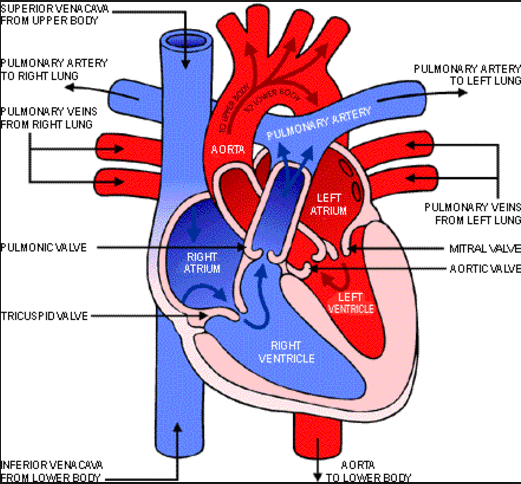
\includegraphics[width=0.9\textwidth]{bilder/b_heart_structure_new}
     \caption{Explaining the decomposition process in a 3 dimensional structured mesh. Illustration taken from \cite{article9}.
     \label{b_heart_structure_new.png}}
\end{figure}

If we were to take our student apartment example even further, the only way of getting into or leaving the lower chambers is by passing the valves. The valves are made of connective tissue [https://www.cardiosmart.org/heart-basics/how-the-heart-works][FOOTNOTE] that acts like flaps. It helps think of the valves as one-way entranced doors that only has two states, open and closed. When the chambers are filled up with blood, and the pressure is greater behind the valve, the cusps (also referred to as leaflets) opens. Similarly, when the pressure is greater in front of the valve, the cusps closes, preventing any blood from flowing backwards. 

The valves can be divided into two types, \textit{semilunar} and \textit{atrioventricular} valves [http://www.biosbcc.net/b100cardio/htm/heartant.htm]. \textit{The atrioventricular valve} (AV) separates the atria from the ventricles. The atrioventricular valves are attached to tough strings called \textit{chordae tendinea} that connects the edges of the \textit{tricuspid} and  \textit{mitral valve} to papillary muscles. When the papillary muscles contract, it effectively prevents the AV from flopping backwards. %%[https://en.wikipedia.org/wiki/Papillary_muscle]
The  AV that separates the RA and RV is the triscupid valve, due to its three cusps. The AV on the left side of the heart is the mitral valve, also called the bicuspid valve, due to its two cusps. 

The semilunar valves (SV) does not have a chordae tendinea to prevent them from overextending, instead the leaflets are shaped like a cup to prevent blood from flowing backwards, and use the blood pressure to close its cusps. The Pulmonic valve is located on the left right side of the heart, while the aortic valve is located on the left side.
%%[http://www.innerbody.com/image/card01.html#full-description].

\begin{figure}[h]
 \centering 
     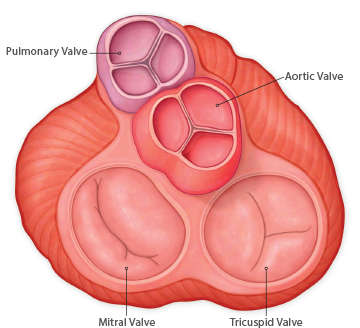
\includegraphics[width=0.9\textwidth]{bilder/b_heart_valves}
     \caption{http://www.medtronic.com/melody/patient/about.html}.
     \label{b_heart_valves.png}
\end{figure}


The right side of the heart consists of a thinner myocardium compared to the left side. The difference in size is related to its functions. The right side of the heart ensures a pulmonary circulation by sending blood to the lungs. The left side of the heart sends blood through the aortic vessel and all the way to the extremeties of the body. Since blood that originates from the left side travels a greater distance compared to the right side, it needs to be sent away with greater force, and thus have a thicker myocardium.

%%If we were to take our student apartment example even further, the only entrance for getting into the left unit is located in the right atrium. This is a one-way entrance, meaning that students can only enter 
%%[http://www.hopkinsmedicine.org/healthlibrary/conditions/
%%cardiovascular_diseases/anatomy_and_function_of_the_heart_valves_90,
%%P03059/]
%%bilde her!


%%the primary function of the cardiovascular system is to supply body cells with nutrient material and carry away waste products
%%, and it does not care about poetry or emotions.

\subsection{The Blood Flow in the Caridovascular System}
An understanding of the circulation of blood through the heart might help the reader to get an better understanding of how the different parts of the heart relate. It helps think of all the blood vessels in the body as a huge sophisticated railway network, where essentially alle the blood in the veins throughout the body ends up in the vena cava, the railway end station. The superior vena cava receives blood from the upper part of the body, whereas the inferior vena cava receives blood form the lower part of the body. As the blood fills up in the RA, the increasingly pressure eventually makes the tricuspid valve shut open, allowing deoxygenated blood [FOOTNOTE] to enter the RV. As the deoxygenated blood flows into the RV, the pressure in front of the tricuspid valve eventually exceeds the pressure behind the valve, resulting in the tricuspid valve to close the cusps. 

As later described in section [X.X] the cardiac cycle includes a contraction followed by a relaxation phase [HEART BOOK]. When the RV contracts, the pulmonic valve opens, allowing deoxygenated blood to enter the pulmonary artery and into the right and left side of the lungs. In the lungs, the carbon dioxide that was added to the red blood cells throughout the body is exhanged for a fresh supply of oxygen.
%%http://www.cts.usc.edu/hpg-valvesoftheheart-circulationofblood2.html
As the LA gets filled with oxygenated blood, the mitral valve will eventually respond to the increasingly pressure behind the valve by allowing blood to enter the LV in the same way as the tricuspid valve. When the LV contracts, the aortic valve opens and the oxygenated blood gets pushed into the artery called the aorta. From the aorta, the freshly oxygenated blood gets sent throughout the body.

By now, the reader should have a basic understanding of how the heart works. Yet one important question remains unanswered, what makes your heart beat?

\subsection{The Electrical Activity in the Cells}
The pumping function of the heart relies on a collective, rhytmic cycle of contraction and relaxation of billions of muscle cells, more specifically, about \(10^{10}\) muscle cells [HEART BOOK]. One of the main reason to why the heart is able to contract and relax is due to the fact that the cardiac cells are excitable, meaning that the cells are able to respond actively to electric stimulus [HEART BOOK]. During the resting phase, the cells are abel to maintain an internal ionic concentration different than those of their surroundings. A cell membrane acts a barrier that sepparates the interior of the cells from the outside environment. A potential difference arises across the cell membrane due to electrically charged ions. The potential difference are referred to as the \textit{transmembrane potential}. The transmembrane potential typically varies from \(-70\) to \(-100\) mV [HEART BOOK] when there is no electric stimulus, also referred to as the resting phase. 

If an eletric stimulus is applied to the muscle cells it results in a change in the potential difference. The cells may react to an potential change, caused by an electric stimulus in one of two ways. If the applied electrical current is too small, the conductive properties of the cell will remain membrane unchanged. When the applied electric stimulus stops, the transmembrane potential quickly returns to its resting state, more specifically, the cells remains its internal negative ionic concentration [HEART BOOK]. If the electrical current is strong enough for the transmembrane potential to reach a certain threshold. It will cause a rappid flux of positive ions into the cell [HEART BOOK]. This phase is referred to as a \textit{depolarization} phase. A depolarization of the membrane causes the transmembrane potential to increase from its negative resting state, to a value around \(0\) mV, or significantly above, depending on the ionic current. The transmembrane potential will gradually return back to its negative resting state, a process referred to as a repolarization of the membrane. The complete process in which a depolarization and repolarization ouccurs, is called an action potential. 

\subsection{Signal Conduction}
The process of electrical signals that propagates throughout the heart, is in the end, the very reason to our existence. The electrical activation of the heart starts in the sinoatrial (SA) node, see figure \ref{b_electrical_heart.png}. The cells in the SA node are what is referred to as self-oscillatory cells. The reason is due to the fact that cells are able to generate electricial current without an external stimulus, more speceifically, as explained in the previous section, they are able to produce action potentials. The frequency of which the action potentials are produced, depends on external factors, such as physical activity level. 
An electrical activation throughout the heart requires a large-scale communication and synchronization between the muscle cells [HEART BOOK]. The electrical activation of the SA-node stimulates neighbouring atrial muscle cells. When one atrial muscle cell is depolarized, the electrical current in the form of ions are able to spread between adjacent cells through protein channels called gap-junctions. The depolarization of one cell therefore affects the potential in neighbouring cells, and may raise the transmembrane potential above the threshold value[HEART BOOK. 

The electrical activation of the heart, hence starts by stimulating a small region of cells in the atria, that results in a propagating wavefront of depolarization across the entire atria, causing the muscle cells to contract. The atria and the ventricles are separated by a non-conductive layer so that the flux of electrical current does not spread directly into the ventricles. Instead, the only way for the electrical signal to be transmitted is through the atrioventricular (AV) node and into the atrioventricular (AV) bundle, as illustrated in figure \ref{b_electrical_heart.png}. The AV-bundle, also referred to as the bundle of His, is a tree-like structure that consists of Purkinje fibers, which provides rapid conduction of the electrical current. The electrical current that passes through the AV-bundle stimulates the ventricular cells at the ends of the Purkinje network. This can be seen from illustration \ref{b_electrical_heart.png}, where the ends of the Purkinje network looks life leaflets in the tree-like structure. As in the case of the atria, the ventricular cells are also connected by gap-junctions. So when the ventricular cells receives a stimulus at the ends of the Purkinje network, it causes a propagating wavefront of depolarized ventricular cells, Which eventually results in a contraction of the entire mass of the ventricles.

The electrical activation of the AV-bundle is quite slow [HEART BOOK]. This results in a small time delay for the electrical signal to reach the ventricles. As a consequence of this delay, the atria contracts, while the ventricles are still relaxed, causing an improvement of the filling of the heart [HEART BOOK].
%%The electrical current are able to spread between adjacent cells through protein channels called gap-junctions.

\begin{figure}[h]
 \centering 
     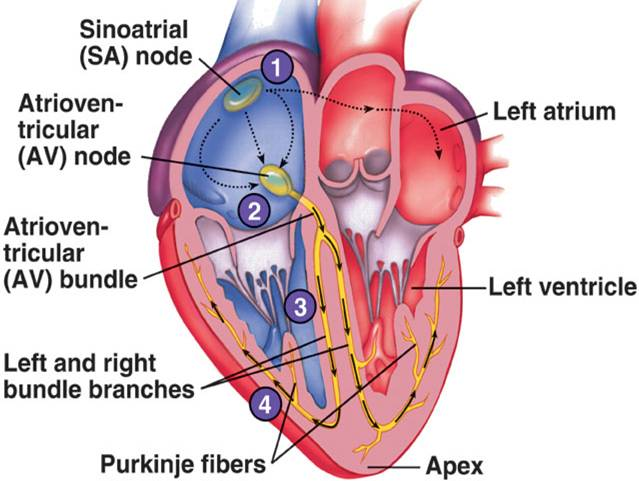
\includegraphics[width=0.9\textwidth]{bilder/b_electrical_heart}
     \caption{http://www.austincc.edu/rfofi/NursingRvw/PhysText/Cardiac.html}.
     \label{b_electrical_heart.png}
\end{figure}


%%which came first, the clot or the heart attack?


%%KILDE: file:///Users/BassE/Downloads/9781461461432-c1.pdf











\section{Multicore Architectures}
\label{sec:multicore_architectures}
Multicore technology is the most important factor that drives today’s microprocessor performance improvements \cite{article6}. The industry has moved away form exponential scaling of clock frequency toward chip multiprocessors (CMP). A modern computer typically consists of several independent CPU cores on the same socket, each having its own cache, and usually a global memory.  

In computer hardware, there are mainly two different types of memory architecture, \textit{shared}, \textit{distributed}, and a hybrid of these two called \textit{distributed shared} memory. Although the memory architectures mentioned above are old concepts and not only bound to multicore architectures, knowing how the processes in a multicore architecture communicates and store data is essential high performance computing. Shared memory refers to a global address space that can be accessed by several different CPUs. Shared memory is easier to program because it offers an unified address space, although, synchronization is needed, and race conditions among the processes can occur. Shared memory architecture can be of two types, \textit{uniform memory access} (UMA) or \textit{non-uniform memory access} (NUMA). A UMA is when all the processors share the physical memory uniformly \cite{article8} meaning that memory access time is uniformly distributed among the CPU cores. A NUMA architecture means that a processor can access its local memory much faster than the non-local memory since each processor has its own system bus for sending and receiving data from memory. A distributed memory system refers to a system in which each processor has its own private memory region, and interaction between different processes happens over an interconnection network. It excludes race conditions and forces the programmer to think about data distribution in the sense that memory is scalable with the number of processing elements, also referred to as \textit{scalability}. every core should access its local memory unit as much as possible to ensure low latency, and a high memory bandwidth. 

\begin{figure}[!h]
  \begin{center}
    \label{b_distributed_memory.png}
    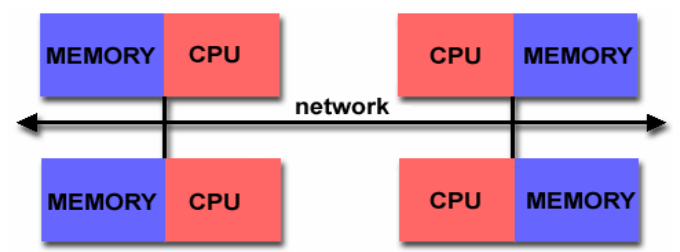
\includegraphics[width=0.45\textwidth]{bilder/b_distributed_memory}
    \label{b_shared_memory.png}
    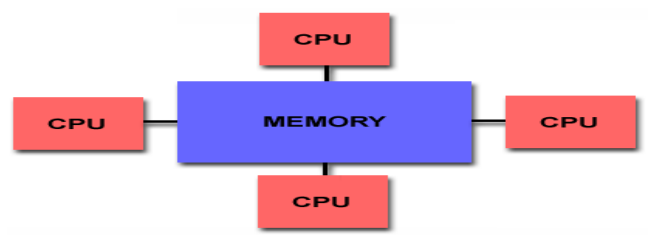
\includegraphics[width=0.45\textwidth]{bilder/b_shared_memory}
  \end{center}
  \caption{overview of distributed and shared memory architecture, respectively. Taken from \cite{article8}}
  \label{b_memory_hierarchy}
\end{figure}

\section{Parallel programming}
\label{sec:problem_decomposition}
\begin{figure}[h]
 \centering 
     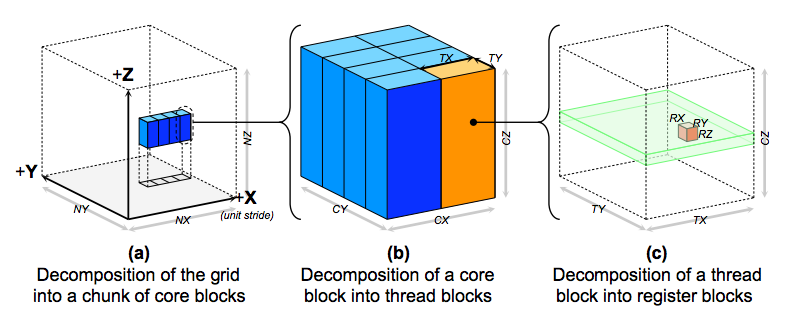
\includegraphics[width=0.9\textwidth]{bilder/b_decomposition}
     \caption{Explaining the decomposition process in a 3 dimensional structured mesh. Illustration taken from \cite{article9}.
     \label{b_decomposition.png}}
\end{figure}
Parallel programming can be split into two categories, shared-memory programming such as Open Multi-Processing (OpenMP), and distributed-memory programming such as the Message Passing Interface (MPI). As discussed in section \ref{sec:multicore_architectures} both memory models have advantages and disadvantages. While OpenMP exploits the shared resources among threads, MPI relies on passing data from one process to another through an interconnection network, each having its own private memory region. In some cases you may want to utilize both programming models, a such technique is often referred to as hybrid parallel programming. In the following example, inspired by \cite{article9}, a hybrid approach can be effectively used to decomposition the problem.

Problem decomposition is one of the most essential stages in a parallel implementation of a problem. Lets assume that we have a large 3D array representing a mesh. To ensure that each processing element gets an equal share of tasks to be executed, we divide the mesh (the entire problem) also referred to as a node block of size \(NX \times NY \times NZ\) into a chunk of core blocks of size (\textit{chunkSize}) \(CX \times CY \times CZ\). By doing so, each process can share its core of blocks. The core blocks are then divided into a series of thread blocks of size \(TX \times TY \times TZ\). Each CPU core usually have multiple threads, decompositioning the problem into thread blocks allows threads to share data which helps reduce capacity misses in the core’s shared cache \cite{article9}. When \( CX = TX\) and \( CY = TY\) there is only one thread per core block. In the third decomposition step, each thread block is then partitioned into register blocks of size \(RX \times RY \times RZ\). Register block optimization involves loop unrolling and jamming, both techniques involves transforming the inner loop. loop unrolling eliminates/reduces data dependency and improves pipelining, while loop jamming reduces loop overhead and gives a better chance for instruction overlap \cite{article10}.
%%explain these, then explain unstructured mesh and why its different
%%To ensure that each processing element gets and equal share of tasks to be executed. 
%%TBD: fine-grained parallelism means that you have a large set of small tasks, which tends to be the case in stencil computation as the mesh size can be complex involving many operations.

%%\subsection{Data Allocation} 

\section{Stencil Computation Overview}
Stencil calculations perform sweeps through data structures that are typically much larger than the available size of the cache. In addition, data reuse is limited to the number of points in the stencil. As a result, many stencil calculations tends to rely on the speed in which data is transferred from memory to the processor. Therefore, effectively use of the hierarchical memory system such as the different levels of cache, proves to be a key factor in stencil computation performance. Reducing communication overhead that occurs while sweeping through the mesh is also essential for high performance, and parallel programming in general.

\subsection{Stencil Iteration Types}
\label{subsec:stencil_iteration_types}
Partial differential equations (PDE) are very important in science and engineering applications. Iterative Methods for solving PDEs has been extensively studied, and in this section I will cover three stencil iteration types, such as Jacobi, Gauss-Seidel, and Gauss-Seidel Red-Black iterations.

\subsubsection{Jacobi}
Iterative methods such as a Jacobi iteration performs a sweep over a mesh, applying a stencil (nearest-neighbor) to each point in the mesh, called the read mesh. Then the result is written to the corresponding point in the second mesh called the write mesh. The Jacobi method performs out-of-place operations, meaning that both read and write operations requires a distinct mesh. A parallel implementation of Jacobi can be done in an embarrassingly parallel fashion \footnote{A straight forward way of parallelizing a problem}, due to any point in the write mesh can be computed independently of each other. A drawback of Jacobi is that it requires to store distinct read and write arrays, resulting in increased memory storage, and the need for more bandwidth.

\subsubsection{Gauss-Seidel}
Gauss-Seidel iterations performs in-place sweeps, meaning that reading and writing to points are done over the same mesh. There can be several read-only meshes, although, a write mesh must be read from first. A drawback from this is that it limits the amount of available parallelism in the sweep, due to almost all the computed stencils will include some points that were already updated during the current sweep, and others that were not. This means that there is an inherent dependency chain that needs to be respected if we wish to replicate the same final answer \cite{article9}. One benefit from using Gauss-Seidel over Jacobi is that both read and write operations are done using the same mesh, thereby reducing the need for additional arrays, creating less memory traffic and storage requirements. 

\subsubsection{Gauss-Seidel Red-Black}
The Gauss-Seidel Red-Black (GSRB) iteration is similar to Gauss-Seidel in the sense that it performs in-place sweeps. To deal with the limited parallelism that the Gauss-Seidel iteration suffers from, a coloring of points are introduced. A black mesh point will only be updated if all the neighboring red points that it depends on have been updated. This process will continue for all the black mesh points. As a consequence, a GSRB iteration only updates every other point. Making this type of sweep similar in parallelism to Jacobi, since every single-color point can be updated independently of each other.

\section{Optimization}
\label{sec:optimization}
Stencil optimization can be divided into two categories, stencil-specific, also referred to as source-level optimization, and compiler based optimizations such as auto-tuning. Following the source-level optimization described in \cite{article9}, we can roughly divide these optimizations into three categories.  Data allocation, bandwidth optimization and kernel optimization. 

\subsection{Bandwidth Optimization}
Improving memory bandwidth is a key factor for optimizing stencil computations. Research paper \cite{article9} introduces two methods for effectively increasing bandwidth. \textit{Software prefetching} aims to hide memory latency by allowing data to be moved into the cache before the data are used, and thereby increase effective memory bandwidth. Another way of increasing memory bandwidth is to reduce memory traffic by using a technique called \textit{cache bypassing}. A cache miss is a failed attempt at read or write a piece of data (also referred to as a cache line) in the cache, which requires access to main memory with much higher latency to get that piece of data, causing a great delay in the overall computation speed. As discussed in section \ref{subsec:stencil_iteration_types}, for a Jacobi iteration performing an out-of-place sweep we are only concerned with the write value being written back to DRAM, since the read data is left unused. As showed in \cite{article9}, getting rid of the extraneous reads for a Jacobi iteration using two meshes, you can eliminate \(\frac{1}{3}\) of the overall memory traffic by removing those cache line allocations, resulting in a 50\% improvement in arithmetic intensity, and if you are bandwidth bound, an increase in performance by up to 50\% \cite{article9}.

\subsection{Kernel Optimization}
Achieving good temporal and spatial locality is a main concern in stencil computation. Temporal locality refers to the reuse of data, if a memory location is referenced, it is most likely to be referenced again in the near future, thus storing and reusing a copy of the referenced data in a low latency, high memory bandwidth like the cache, yields better performance. Spatial locality refers to the use of neighboring data items. If a memory location is referenced, it is most likely that nearby memory locations will be referenced in the near future \cite{article14}.

as discussed in section \ref{sec:problem_decomposition}, and implemented in \cite{article1}, register blocking involves loop transformations like unroll and jam. There are numerous other ways of optimizing a loop. Following the examples given in \cite{article10} we have \textit{loop interchange}, which involves exchanging the inner loop with the outer loop. This may improve the spatial and temporal locality. Reducing nested loops into a single-nested loop, also known as \textit{loop collapsing} may reduce loop overhead and improve run-time performance \cite{article11}. Another loop transformation technique named \textit{loop peeling} involves performing a problematic iteration separate before entering the loop, with the aim at eliminating dependencies or simplifying a loop. Other loop optimizations can be found in \cite{article12}.

\subsection{Auto-tuning}
Now that we have explored a variety of stencil specific optimizations, it is time to move on to compiler based optimization such as auto-tuning. Auto-tuners evaluates a large optimization space by generating variants of a given kernel, as discussed in section \ref{sec:optimization}, and benchmarking its performance. The search effectively tries all the optimizations and reports both peak performance and the most optimal parameters. Auto-tuning is not a new concept and existing libraries include ATLAS and FLAME for dense linear algebra, which involves dot product and matrix multiplication. The sparse linear algebra library OSKI, which involves sparse matrix-vector multiplication (SpMV), and Spiral for spectral methods. The auto-tuning environment created in \cite{article1} encompasses most of the stencil optimizations described in this essay, notably, their optimized stencil is 1.5\(\times\)-5.6\(\times\) faster than the naive parallel implementation, and with a median speedup of 4.1\(\times\)  on cache based architectures \cite{article1}.

%%\subsection{Optimization on Unstructured Meshes}
%%\label{subsec:optimization_on_unstructured_meshes}
%%While most research has been devoted to stencil computation over structured meshes, the need for more accurately discretizing complex geometries has led to a rise in the use of unstructured mesh techniques \cite{article2}, \cite{article13}. Most stencil optimization techniques in a regular application consist of exploiting the regular geometric memory access pattern to achieve high performance and maximize the parallelism. Numerical operations over an unstructured mesh tends to yield lower performance and parallelism, due to the different geometric patterns based on the centered point in the stencil. Proved in research paper \cite{article4}, the key to high performance for unstructured tetrahedral meshes lies in a reordering of the tetrahedra, such that the resulting connectivity matrix resembles a block diagonal form where the optimal size of the blocks depends on the hardware \cite{article4}, meaning that carefully fitting the blocks of data in the cache is essential for high performance.

%%Research paper \cite{article2} presents two strategies for evaluating stencil computation over a 2D unstructured triangular mesh, \textit{per-point} and \textit{per-element}. The per-point method iterates over a mesh, and for each point finds all of the triangles that intersect with the stencil centered around that point. The per-element method iterates over a mesh, and for every triangle finds all of the points whose stencil intersects with that triangle \cite{article2}. These two methods tries to maximize data-reuse and data locality. \cite{article2} also claims that the 2D solutions over an unstructured mesh can be extended to 3D unstructured tetrahedral meshes.

%%\section{Related Work}
















